\documentclass[12pt, a4paper]{report}
\usepackage{amsmath,amsthm,amsfonts,amssymb,amscd}
\usepackage[table]{xcolor}
\usepackage[margin=2cm]{geometry}
\usepackage{graphicx}
\usepackage{multicol}
\usepackage{mathtools}
\usepackage{palatino}
\usepackage[utf8]{inputenc}
\usepackage[brazil]{babel}
\usepackage[pdftex]{hyperref}
\usepackage{lettrine}
\usepackage{float}
\usepackage{caption}
\usepackage{subcaption}

\renewcommand*{\ttdefault}{txtt}
\newlength{\tabcont}
\setlength{\parindent}{0.0in}
\setlength{\parskip}{0.05in}

\begin{document}
	
	\chapter*{Resumo}
	\chapter*{Abstract}
	\chapter{Introdução}
	
	\chapter{Ontologias}
\label{chap:ontologias}

\lettrine{A}{} palavra Ontologia veio do grego, assim como vários outros termos que se referem a alguma área de estudo. Seu significado, no entanto, é muito mais abstrato. Diferentemente de Biologia, que é "o estudo da vida", a palavra cujo plural dá nome a este capítulo quer dizer "o estudo do ser enquanto ser". O dicionário Merriam-Webster \cite{ontoMerriam} estende essa definição como: "um ramo da metafísica preocupado com a natureza e as relações do ser".

Importado da Filosofia, esse conceito começa a ser trabalhado muito antes da época dos computadores. Aristóteles já estudava Ontologia em suas Categorias \cite{ontoDahlberg}. No entanto, apenas em 1606, com o livro \textit{Ogdoas Scholastica}, de Jacob Lorhard, foi que a palavra em si realmente surgiu. Esse termo ficou popular em 1729 com o livro \textit{Philosophia Prima: sive Ontologia}, de Christian Wolff, com a definição "\textit{Ontology or First Philosophy is the science of Being in general or as Being}" \footnote{"Ontologia ou Filosofia Primeira é a ciência do ser em real ou como um ser."} \cite{ontoNickles}.

Para a Ciência da Computação, a definição é um pouco diferente, embora possua muita semelhança com o conceito já explícito. Guarino \cite{ontoGuarino} definiu ontologia como "um artefato de engenharia, constituído por um vocabulário específico usado para descrever uma certa realidade, mais uma série de pressupostos explícitos acerca do significado que se atribui a esse vocabulário". Logo, uma ontologia seria uma reunião de sentenças lógicas que exibem alguma informação sobre alguma área do mundo para resolver algum problema relacionado a ela.

Fazendo um paralelo entre ambas as disciplinas, pode-se observar que, enquanto a primeira faz um estudo sistemático da existência, na segunda existe um foco maior em o que pode ser representado.

As ontologias são estudadas na área de Inteligência Artificial, que está preocupada com a automação do comportamento inteligente. Na prática, elas funcionam como um sistema "\textit{tell and ask}". Algumas coisas são contadas para os agentes inteligentes (uma entidade autônoma com comportamento que simula inteligência), e então, perguntas podem ser feitas para eles, embora não precisem saber todas as respostas. 

Surgiram de um contexto onde os cientistas desejam modelar e representar o mundo para as máquinas, e isso ocorre desde a origem dos computadores. Como cada pessoa possui uma visão de mundo, cada modelagem será diferente de algum jeito. Por isso, a construção de ontologias é um tópico que merece estudo. Atualmente, esta área é bastante pesquisada por sua aplicação com Web Semântica. 

As ontologias denotam uma "especificação explícita de uma conceitualização" \cite{ontoGruber}, e, uma vez construídas, permitem comunicação, compartilhamento e reúso de conhecimentos. Elas interessam várias áreas do conhecimento, tais como a ciência da computação, filosofia, engenharia de dados, \textit{data science}, lógica e linguística.

\section{Definições preliminares}

Smith \cite{ontoSmith} definiu alguns conceitos que nos auxiliam a compreender melhor o que é uma ontologia.

\begin{description}
	\item[Representação] Seria uma ideia, uma imagem, um registro, ou uma descrição que se refere, ou é sobre, ou pretende referir a alguma entidade externa à representação.
	\item[Representação Composta] É uma representação constituída de sub-representações como as suas partes, da mesma maneira em que os parágrafos são feitos de sentenças e as sentenças de palavras. A menor sub-representação se chama unidade representacional, que pode ser um ícone, um símbolo, um nome, entre outros.
	\item[Representação Cognitiva] É uma representação cujas unidades representacionais são ideias, pensamentos ou crenças na mente de algum sujeito pensante.
	\item[Artefato Representacional] É uma representação fixa em algum meio de modo que pode servir para fazer representações cognitivas que existem em mentes separados. Exemplos: um texto, um diagrama, um mapa, uma lista, entre outros.
	\item[Porção de Realidade] Termo que compreende universais únicos e particulares e suas com\-bi\-na\-ções mais ou menos complexas.
	\item[Domínio] É uma porção da realidade que forma o assunto de estudo de uma ciência ou tecnologia. Ex: Radiologia, História, Arqueologia, etc..
	\item[Taxonomia] É um artefato representacional em um grafo na forma de árvore com os nós representando universais ou classes e as arestas sendo relações "\textit{is-a}" ou "\textit{part-of}", que serão tratadas mais adiante.
	\item[Ontologia] É um artefato representacional que compreende uma taxonomia própria, cujas unidades representacionais são usadas para designar uma combinação de universais, classes definidas e relações entre eles.
\end{description} 

\section{Conceitualização}
	
Existe um certo debate sobre a definição de Conceitualização. Depois de propor o que era uma ontologia, Gruber sugeriu que uma Conceitualização "é uma visão abstrata e simplificada do mundo que se quer representar para algum propósito". Essa definição parece boa, mas deixa algumas pontas soltas. O que seria uma "visão", por exemplo, deixa algumas dúvidas.

Para Guarino e Giaretta \cite{ontoGiaretta}, uma Conceitualização pode ser entendida como “uma estrutura semântica intensional que codifica as regras implícitas que determinam a estrutura de uma porção da realidade”. Essa definição é um pouco mais concreta, e já é possível pensar sobre ela computacionalmente.

Pode-se inferir que uma Conceitualização é uma modelagem de parte de algum domínio do conhecimento. O domínio nada mais seria do que alguma disciplina, como a Geografia, Música, Enologia, entre outros. Tal modelagem é feita a partir de alguma linguagem formal de representação (em geral, Lógicas de Descrição) e deve levar em conta a generalidade que se aplica ao domínio escolhido.

Vale lembrar que, embora sejam amplamente utilizadas na vida real, as linguagens naturais não são consideradas linguagens formais. Isso tem uma explicação simples. Basta lembrar das figuras de linguagem, como a metáfora e o eufemismo, amplamente usadas nos discursos escrito e falado. 

Debruyne \cite{ontoDebruyne} fez um estudo mais sistemático sobre o que seria uma Conceitualização, baseado na pesquisa de Guarino \cite{ontoGuarino}. Para facilitar o entendimento das definições que virão a seguir, é necessário entender dois conceitos vindos da Filosofia:

\begin{description}
	\item[Contexto Intensional] Ocorre quando um termo não pode ser substituído sem que a verdade sobre a sentença seja ameaçada. Por exemplo, embora saibamos que Clark Kent é o Super-Homem e também é um jornalista, a sentença a seguir é falsa, pois o Super-Homem não é um jornalista:
	\begin{itemize}
		\item Lois Lane acredita que o Super-Homem irá investigar uma notícia com ela. 
	\end{itemize}
	\item[Contexto Extensional] Se refere à extensão de um termo, que é o conjunto de objetos que ele denota. Um contexto é extensional se alguma expressão $ e $ aparece e pode ser substituída por uma expressão com a mesma extensão mantendo o seu valor verdadeiro. Por exemplo: 
	% e'
	\begin{itemize}
		\item Violão é um instrumento musical.
		\item Piano é um instrumento musical.
	\end{itemize}
	Acima, temos que \textit{instrumento musical} é uma extensão de \textit{Violão} e de \textit{Piano}.	
\end{description}

Feito este esclarecimento, seguem as definições de Guarino.

\begin{description}
	\item[Noção Extensional de Conceitualização] É um par $(D,R)$, onde $D$ é um domínio e $R$ são as relações relevantes que existem nesse domínio.
	\item[Espaço Domínio] Um par $(D,W)$, com $ D $ representando um domínio e $ W $ sendo os mundos possíveis dentro dele, ou seja, os conjuntos máximos de estados das coisas desse domínio.
	\item[Relação Conceitual] Dado um espaço domínio $ (D,W) $, uma relação conceitual $ \rho^n $ de aridade $ n $ em $ (D,W) $ é definida como uma função total $ \rho^n : W \to 2^{D^n}$ de $ W $ para o conjunto de todas as relações $ n $-árias em $ D $.
	\item[Noção Intensional de Conceitualização] Uma Conceitualização para $ D $ é definida como uma tripla ordenada $ C=(D,W,R) $, onde $ R $ é um conjunto de relações conceituais do espaço domínio $ (D,R) $. \\ \\
	Definindo uma Linguagem Lógica $ L $ com um Vocabulário $ V $, teremos:
	\item[Interpretação Extensional de uma Linguagem] Um modelo para $ L $ é definido como uma estrutura $ (S,I) $, onde $ S=(D,R) $ é uma estrutura de mundo e $ I : V \to D \cup R $ é uma função de interpretação atribuindo elementos de D para símbolos constantes de $ V $ e elementos de $ R $ para símbolos predicados de $ V $.
	\item[Interpretação Intensional de uma Linguagem] Por meio de uma estrutura $ (C, I) $, onde $ C $ é uma Conceitualização como definido no item 3, e $ I $ é uma função de interpretação como definido no item acima, teremos que uma interpretação intensional é um compromisso ontológico $ K $ para $ L $. 
	\item[Conjunto de modelos pretendidos de uma linguagem de acordo com um compromisso] \hfill \\ O conjunto $ I_K(L) $ de todos os modelos pretendidos de uma linguagem $ L $ que são compatíveis com um compromisso $ K = (C,I) $ são todos os modelos de $ L $ que são compatíveis com $ K $. O compromisso garante consistência.
\end{description}

\section{Construindo uma ontologia}

Para construir uma ontologia, é necessário escolher um domínio e o nível de generalidade que é necessário que ela atinja. Também deve-se ter em mente quem vai usá-la. Para que ela alcance o máximo de utilidade, é necessário que as perguntas que se deseja que ela responda sejam feitas antes de sua construção.

Geralmente, grandes ontologias são projetadas por equipes interdisciplinares, para que ela seja o mais correta e abrangente quanto possível. Quando se confecciona uma Ontologia, é necessário que sejam feitas algumas decisões de projeto.  

Gruber \cite{ontoGruber} fez uma proposta de critérios de \textit{design} para ontologias com o objetivo de tornar o compartilhamento de conhecimento e interoperabilidade com programas baseados em conhecimento mais fácil. Eles são os seguintes:

\begin{description}
	\item[Clareza] Uma ontologia deve ter uma linguagem clara e efetiva na definição de seus termos. Tal definição deve ser objetiva. Embora ela possa vir de situações sociais ou requisitos computacionais, ela deve ser independente destes contextos. Usar uma linguagem lógica, é um meio para este fim, ou seja, quando for possível fazer uma definição usando axiomas lógicos, isso deve ser feito. Onde possível, uma definição completa (com condições necessárias e suficientes) é preferível a uma definição parcial (com condições necessárias ou suficientes). Todas devem ser documentadas usando linguagem natural.
	\item[Coerência] Uma ontologia deve permitir inferências consistentes com suas definições. No mínimo, os axiomas usados nas definições devem ser logicamente consistentes. A coerência também deve ser aplicada aos conceitos informais, definidos na linguagem natural da documentação e nos exemplos. Se uma sentença que pode ser inferida contradiz uma definição ou exemplo dado informalmente, a ontologia é incoerente.
	\item[Estendibilidade] Uma ontologia deve ser projetada para ser capaz de antecipar o uso de conhecimento compartilhado. Ela deve oferecer uma fundação conceitual de modo que o novo conhecimento possa ser apoiado nela e que a ontologia possa ser estendida e especializada, ou seja, novos termos podem ser definidos usando o vocabulário existente, de modo que a revisão das crenças do conhecimento anterior possa ser evitada ao máximo.
	\item[Viés mínimo de codificação] A Conceitualização deve ser especificada num nível de conhecimento que não dependa de uma codificação que utiliza um nível de símbolos particulares. Um viés de codificação ocorre quando as escolhas de representação são feitas por pura conveniência de notação ou de implementação. Como agentes de conhecimento podem ser implementados em diferentes sistemas e estilos de representação, isso deve ser minimizado.
	\item[Compromisso ontológico mínimo] Isso faz com que ela suporte as atividades de compartilhamento de conhecimento desejadas. Quanto menos suposições sobre o mundo modelado, melhor. Isso permite que as partes comprometidas com a ontologia sejam livres para especializar e instanciar a ontologia o quanto quiserem. Já que isso é baseado no uso consistente do vocabulário, ele pode ser minimizado usando uma teoria fraca (genérica) e definindo apenas os conceitos necessários para a comunicação do conhecimento consistente com esta teoria.
\end{description}

É possível notar que todos esses critérios não poderão ser atendidos ao mesmo tempo, portanto, alguns \textit{trade-offs} deverão ser feitos.
Podemos ter um conflito, por exemplo, entre os critérios 1 e 3, já que o máximo de clareza implica que as definições terão a sua interpretação restrita.

\subsection{Componentes de uma ontologia}

Computacionalmente falando, as ontologias possuem cinco partes. Para ilustrá-las melhor, vamos fazer uma ontologia sobre Música. Será usada uma fonte monoespaçada para as partes dela.

\begin{description}
	\item[Classes] Descrevem os conceitos de um certo domínio do discurso. São o foco das ontologias. São uma coleção de todos os particulares aos quais é possível aplicar um termo geral. Por exemplo: a classe \texttt{Cantor}.
	\item[Propriedades] São atributos que descrevem características do conceito a que uma classe se refere. Em nosso exemplo, a classe \texttt{Cantor} possui as propriedades \texttt{Nome}, \\ \texttt{RitmoPredominante} e \texttt{Idade}.
	\item[Relações] Ontologias são constituídas de relações hierárquicas. Por exemplo \texttt{Cantor} $ \to $ \texttt{Pessoa}. A hierarquia de classes representa uma relação “\textit{is-a}”\cite{ontoFranca}. Tais relações são transitivas. Existem também as relações "\textit{part-of}", que já estão dentro da Teoria dos Conjuntos. Uma classe é parte da outra se a compõe.
	\item[Restrições] São os tipos das propriedades, por exemplo: enquanto para \texttt{Nome} e \\ \texttt{RitmoPredominante} uma \textit{string} seja suficiente, para a Idade, um inteiro já está de bom tamanho.
	\item[Instância] é um indivíduo (por exemplo, \texttt{MariahCarey}), de um conjunto universal (cantores, músicos, pessoas). Vale lembrar que uma instância não é uma subclasse.
\end{description}

Como já vimos acima, uma classe pode ter nomes diferentes, pois não é ele que define uma classe. Sinônimos e palavras em línguas distintas não representam classes diferentes.

Várias classes subordinadas a uma superclasse são consideradas irmãs. Elas devem ter o mesmo nível de generalidade. Por exemplo, seja uma classe \texttt{Musica}. Suas subclasses podem ser \texttt{Cancao} e \texttt{MusicaAmericana}, e não \texttt{Cancao}, \texttt{MusicaAmericana} e \texttt{MusicaBrasileira} (a última é subclasse da penúltima).

Os conceitos definidos até aqui mostram um jeito de caracterizar ontologias, que é pelo número de termos que ela possui. Uma outra métrica é o número de axiomas lógicos que ela possui. 

Existem três processos para definir as classes e a hierarquia, a seguir:

\begin{description}
	\item[\textit{Top-down}] Vai das classes mais genéricas para as mais específicas. Um exemplo seria criar os ritmos gerais e depois aprofundar para os regionais.
	\item[\textit{Bottom-up}] Vai das classes mais específicas para as mais genéricas, agrupando as específicas já criadas. Na ontologia estudada aqui, seria possível começar dos ritmos regionais e depois agrupá-los por suas semelhanças.
	\item[Vai-e-Vem] Define conceitos simples para generalizá-los e especificá-los. Seria uma com\-bi\-na\-ção dos dois primeiros itens.
\end{description}

\subsection{Montando a ontologia}

Montar uma ontologia é um processo que segue os seguintes passos:

\begin{itemize}
	\item Definir as classes da ontologia.
	\item Colocá-las em uma hierarquia taxonômica.
	\item Determinar suas propriedades e restrições.
	\item Criar uma base de conhecimento para essas classes e propriedades, ou seja, preencher a ontologia com as instâncias.
	\item Colocar os valores das propriedades para as instâncias.
\end{itemize}

Embora pareça ser direto, esse processo é iterativo, como afirmam Noy e McGuinness \cite{ontoNoy}. Uma vez feito, deve ser repetido para que haja uma adequação das classes com as instâncias colocadas, pois, por exemplo, se uma classe acabar com apenas uma subclasse, a modelagem pode ter um problema, ou a ontologia não está completa. E ainda, se uma classe possui mais de uma dúzia de subclasses, novas categorias (classes ou subclasses) podem ser necessárias. 

Às vezes, uma classe possui muitas propriedades específicas e diferentes em várias de suas instâncias. Nesse caso, a inserção de uma classe deixará a ontologia mais compreensível. A nova classe fará com que a distinção das instâncias ocorra, efetivamente, evitando mal-entendidos.

Teoricamente, o processo nunca acaba. Na prática, ele é interrompido quando a ontologia fornece respostas suficientemente boas para a maior parte das consultas realizadas, ou seja, tal critério é subjetivo.

Ainda em relação às classes, algumas observações podem ser feitas. A primeira é em relação à herança múltipla. Ela acontece quando uma classe é subclasse de várias outras classes, por exemplo, a classe \texttt{PopBrasileiro}, pode pertencer à classe \texttt{Pop} e à classe \texttt{MusicaBrasileira}. Isso é aceitável, pois no mundo real, acontece várias vezes e de diversas maneiras.

Outro aspecto interessante é o de Classe Abstrata. Uma classe desse tipo não pode ter instâncias diretas. Em nossa ontologia, podemos ter classes de músicas regionais. A classe \texttt{Musica} pode ter varias subclasses, tais como \texttt{MusicaArgentina} e \texttt{MusicaBrasileira}, entre outras. Note que essas classes são abstratas, pois no mundo real, não existe mais de um tipo de Música Brasileira, como um conjunto de ritmos, que possa pertencer ao conceito \texttt{MusicaBrasileira}.

As ontologias possuem suporte a classes disjuntas. Classes disjuntas são aquelas que não possuem uma intersecção. Em nossa ontologia, \texttt{Cantor} e \texttt{Compositor} não são disjuntas. No entanto, \texttt{Cancao} e \texttt{HinoNacional} são classes disjuntas.

Para os nomes das classes, não há uma convenção específica, só há um consenso de manter um padrão de nomenclatura é algo bom. Para fazer isso, pode-se usar \texttt{snake\textunderscore case}, \texttt{camelCase} ou usar espaços na grafia. Além disso, deve-se prestar atenção se o nome de uma classe possui o nome de sua superclasse ou não.

Uma ontologia não precisa ter toda a informação existente sobre o domínio. Não é necessário especializar ou generalizar mais do que seja necessário para a aplicação. Além disso, as classes não precisam ter todas as propriedades possíveis e nem carregar todas as distinções que estão no mundo. Isso significa que a ontologia deve ser o modelo mais simples para o problema que se deseja resolver.

Algumas relações podem ter uma inversa, assim como ocorre com funções matemáticas. Uma relação que possui uma inversa pode ser:

\begin{itemize}
	\item \texttt{Cantor canta Musica}
	\item \texttt{Musica cantadaPor Cantor}
\end{itemize}

\section{Usabilidade de uma ontologia}

A criação de uma ontologia é feita por uma equipe interdisciplinar, geralmente composta por \textit{experts} da área que se deseja cobrir e técnicos para a confecção de ontologias (vindos da área de Computação). Isso não limita a equipe de possuir profissionais de mais áreas. Uma ontologia é feita para que qualquer pessoa possa acessar suas informações.

É possível achar os usuários de uma ontologia, mas nem sempre o seu autor. O razoável é assumir que elas foram evoluindo com o passar do tempo. 

Ontologias feitas sobre áreas de estudo (por exemplo, a Aviação) serão muito mais úteis do que aquelas feitas sobre acontecimentos (como a queda do voo TAM 3054). A existência dessa última nem faz sentido, já que as ontologias servem para modelar casos gerais, não particulares. Seria melhor, por exemplo, construir uma ontologia sobre acidentes de avião e seus conceitos.

\section{Problemas relacionados}

Existem alguns problemas relacionados a ontologias. Os mais comuns são os problemas de modelagem e construção. Um problema muito comum é a existência, na linguagem natural, de Homônimos e Sinônimos. Deve existir um cuidado especial com eles, já que eles podem levar a uma confusão na nomenclatura.

Em relação à modelagem, o problema de não utilizar uma equipe interdisciplinar especializada pode levar a uma cobertura incompatível de conceitos, ou seja, as classes podem ficar muito distantes da realidade. Além disso, usar fontes não confiáveis na ontologia pode fazer com que os problemas que elas estavam sendo feitas para resolver, não sejam resolvidos corretamente.

Tais problemas tornam-se muito maiores quando duas ontologias são integradas. A possível integração entre ontologias é um dos motivos para elas existirem, afinal, isso pode acelerar o seu desenvolvimento. Em nosso exemplo, se já existir uma ontologia sobre Música Brasileira, poderemos absorvê-la, mas o cuidado terá de ser redobrado em relação às questões acima. 

Em relação à implementação, os pontos que surgem são em geral a respeito da linguagem utilizada, mas isso será tratado no \autoref{chap:logicas}.

Além dos já citados, pode acontecer de chegar um novo conhecimento e a ontologia ficar inconsistente. Neste caso, terão de ser usadas algumas operações de Revisão de Crenças, foco deste trabalho, que será estudado no \autoref{chap:revisao}.

A ontologia construída nesse capítulo fica assim: 

\begin{figure}[H]
	\centering
	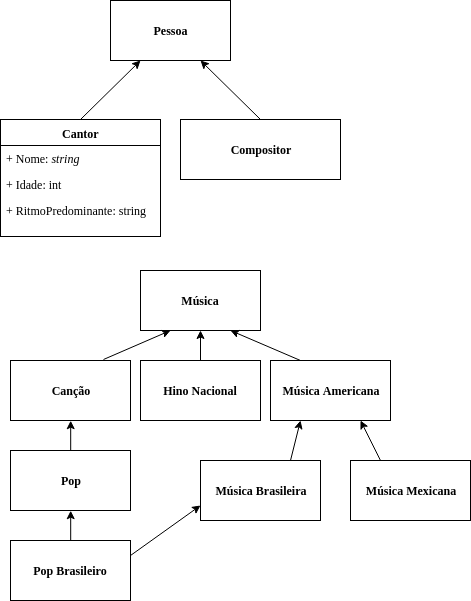
\includegraphics[width=0.6\textwidth]{Capitulos/Ontologias/OntologiaMusica}
	\caption{Esquema de classes de uma ontologia sobre Música}
\end{figure}
	\chapter{Lógicas de Descrição}

\lettrine{A}{} área de Inteligência Artificial é composta por diversas subáreas, que são responsáveis por diversos estudos. Uma delas é a de Representação de Conhecimento, que cuida de construir formalismos adequados para expressar conhecimento sobre um domínio. Tal área tem seus estudos válidos, afinal, entidades inteligentes possuem algum tipo de conhecimento e precisam fazer inferências a partir dele.

Existe um consenso, já mencionado no capítulo anterior, de que linguagens formais são uma maneira boa de caracterizar axiomas lógicos para a modelagem de uma ontologia. O principal formalismo utilizado para representar conhecimento, com um cuidado especial para as terminologias, são as Lógicas de Descrição (doravante, LD).

Essas lógicas são um subconjunto da Lógica de Primeira Ordem (a partir de agora, LPO), que por sua vez, estende a Lógica Proposicional. As LD são utilizadas por sua expressividade. Para anotar que uma \texttt{Cancao} ou um \texttt{HinoNacional} são uma \texttt{Musica}, usando a ontologia que está sendo desenvolvida neste trabalho, podem ser utilizadas as seguintes sentenças, usando as lógicas até agora citadas:

\begin{table}[H]
	\centering
	\begin{tabular}{|l|l|l}
		\cline{1-2}
		Lógica                           & Sentença                                                                             & \\ \cline{1-2}
		Proposicional                    & $c \lor h \to m$                   & \\ \cline{1-2}
		de Primeira Ordem                & $\forall x(\texttt{Cancao}(x) \lor \texttt{HinoNacional}(x) \to \texttt{Musica}(x))$ & \\ \cline{1-2}
		de Descrição ($ \mathcal{ALC} $) & \texttt{Cancao} $\sqcup$ \texttt{HinoNacional} $\sqsubseteq$ \texttt{Musica}         & \\ \cline{1-2}
	\end{tabular}
\caption{A mesma sentença expressa em diferentes lógicas}
\end{table}

Podemos observar que a notação da LD permite que a interpretação de suas sentenças seja feita usando a Teoria dos Conjuntos. Na última sentença da tabela, é possível inferir que a união dos conjuntos \texttt{Cancao} e \texttt{HinoNacional} está contida no conjunto \texttt{Musica}.

\section{Conceitos, papéis e indivíduos}

As LD possuem um jeito próprio de organizar o conhecimento. Elas usam três definições para retratar o que é desejado \cite{logicaMatos}. Cada uma delas é utilizada na construção de uma ontologia. São, a seguir:

\begin{itemize}
	\item Conceitos: Também chamados de classes, representam um conjunto de indivíduos. Nas ontologias, são equivalentes às Classes.
	\item Papéis: Podem ser denotados como propriedades. Retratam as relações binárias que existem entre os indivíduos. Basicamente, são as Relações de uma ontologia. Alguns papéis podem ter uma função de caracterização, ou seja, definindo alguns atributos para o conceito. Tal função corresponde a uma Propriedade de uma Classe, em uma ontologia.
	\item Indivíduos: Representam os particulares que existem dentro de um Conceito. Para as ontologias, são as Instâncias.
\end{itemize}

Logo, uma LD é definida por uma tripla $ (N_C, N_R, N_I) $, onde $ N_C $ é um conjunto de Conceitos atômicos, $ N_R $ é um conjunto de Papéis atômicos e $ N_I $ é um conjunto de nomes de indivíduos.

Feita essa distinção, o conhecimento em uma ontologia é dividido em duas partes, com as LD. A primeira delas é a \textit{TBox}. Ela se refere ao conhecimento terminológico, ou seja, o conhecimento intensional do domínio. Nela ficam os conceitos, as propriedades e as restrições.

A outra parte é a \textit{ABox}, e nela fica o conhecimento assertivo, ou seja, o conhecimento extensional. Ela contém as asserções sobre as instâncias, ou seja, como eles se encaixam nas definições explícitas na \textit{TBox}.

\section{$\mathcal{ALC}$ e outras linguagens}

As pesquisas na área de Representação de Conhecimento levaram à confecção das chamadas Linguagens Terminológicas de Representação. Uma delas é a KL-ONE de Brachman, que possui uma semântica clara, além de separar o conhecimento assertivo e terminológico. %Citar o home

Tais estudos levaram ao desenvolvimento da $\mathcal{ALC}$. Essa linguagem, cuja sigla significa \textit{Attributive Concept Language with Complements}, é uma das Lógicas de Descrição mais básicas que existem, embora seja uma das mais utilizadas para as atividades que envolvem raciocínio lógico. 

Ela contempla os seguintes construtores, para quaisquer conceitos \texttt{A} e \texttt{B} e qualquer papel \texttt{r}:

\begin{table}[H]
	\centering
	\begin{tabular}{|c|c|l}
		\cline{1-2}
		Nome        & Notação                               &  \\ \cline{1-2}
		Conceito Universal      & $ \top $                            &  \\ \cline{1-2}
		Conceito Vazio      & $ \bot $                            &  \\ \cline{1-2}
		Conceito Atômico      & \texttt{A}                            &  \\ \cline{1-2}
		Negação      & $ \neg $\texttt{A}                            &  \\ \cline{1-2}
		União       & \texttt{A} $ \sqcup $ \texttt{B}      &  \\ \cline{1-2}
		Intersecção & \texttt{A} $ \sqcap $ \texttt{B}      &  \\ \cline{1-2}
		Universal   & $\forall$ \texttt{r.A}                &  \\ \cline{1-2}
		Existencial & $\exists$ \texttt{r.A}                &  \\ \cline{1-2}
	\end{tabular}
	\caption{Construtores da Lógica $ \mathcal{ALC} $}
\end{table}

Essa representação também permite que sejam escritos axiomas terminológicos, tais como a subsunção, denotada por $ \texttt{A} \sqsubseteq \texttt{B} $, e a equivalência, caracterizada como $ \texttt{A} \equiv \texttt{B} $ e que significa $ \texttt{A} \sqsubseteq \texttt{B} $ e $ \texttt{B} \sqsubseteq \texttt{A} $. Para o conhecimento assertivo também existem axiomas, tanto para conceitos ($\texttt{A}(x)$), quanto para papéis ($\texttt{r}(x,y)$).

A linguagem $\mathcal{ALC}$ permite que seja feita a negação de conceitos complexos (não-atômicos). Tal propriedade permite descobrir, por exemplo, se algum conceito é satisfatível. Usando o símbolo $ \sim $ para demonstrar equivalência, teremos que:

\begin{itemize}
	\item $ \neg(\forall r.\texttt{A}) \sim \exists r.\neg \texttt{A}$ 
	\item $ \neg(\exists r.\texttt{A}) \sim \forall r.\neg \texttt{A}$ 
	\item $ \neg(\texttt{A} \sqcup \texttt{B}) \sim \neg \texttt{A} \sqcap \neg \texttt{B}$ 
	\item $ \neg(\texttt{A} \sqcap \texttt{B}) \sim \neg \texttt{A} \sqcup \neg \texttt{B}$ 
	\item $ \neg \neg \texttt{A} \sim \texttt{A} $
\end{itemize}

A partir de sua constituição, é possível definir três sublinguagens da $\mathcal{ALC}$ \cite{logicaSchmidt}, que são descritas a seguir.

\begin{itemize}
	\item $\mathcal{ALE}$: permite a descrição de conceitos simples sem a utilização de uniões; 
	\item $\mathcal{ALU}$: deixa apenas conceitos simples serem descritos e restringe as quantificações de papéis existenciais à forma $ \exists\texttt{r}.\top $;
	\item $\mathcal{AL}$: é a intersecção das sublinguagens acima.
\end{itemize}

Os nomes das sublinguagens acima são derivados da seguinte maneira: $ \mathcal{ALU} $ vem da junção de $ \mathcal{AL} $ com uniões, $ \mathcal{ALE} $ é a $ \mathcal{AL} $ acrescida de quantificadores existenciais. A própria $ \mathcal{ALC} $ é uma extensão da $ \mathcal{AL} $ com adição de complementos (negações) para qualquer conceito, seja ele atômico ou complexo. 

Nota-se que a sigla que representa o nome de uma linguagem expressa as características que ela possui.
A $ \mathcal{ALC} $ é base para outras linguagens mais expressivas, que são construídas a partir de sua extensão. Algumas delas são:

\begin{itemize}
	\item $ \mathcal{S} $: linguagem $ \mathcal{ALC} $ com papéis transitivos;
	\item $ \mathcal{F} $: propriedades funcionais;
	\item $ \mathcal{N} $: restrição numérica;
	\item $ \mathcal{C} $: negação de conceitos complexos;
	\item $ \mathcal{U} $: união de conceitos;
	\item $ \mathcal{E} $: quantificação existencial completa;
	\item $ \mathcal{Q} $: restrição numérica qualificada;
	\item $ \mathcal{O} $: nominal;
	\item $ \mathcal{H} $: hierarquia de papéis;
	\item $ \mathcal{I} $: propriedades inversas;
	\item $ \mathcal{N} $: restrições de cardinalidade;
	\item $ ^\mathcal{(D)} $: usa propriedades de tipo de dados.
\end{itemize}

Com essa nomenclatura, pode-se dar duas linguagens como exemplo\cite{logicaResina}. Uma delas é a $ \mathcal{SHIF}^\mathcal{(D)} $, que engloba a $ \mathcal{ALC} $ e, ainda, hierarquia de papéis, propriedades inversas, transitivas e funcionais e tipos de dados.

Uma outra é a lógica $ \mathcal{SHOIN}^\mathcal{(D)}$, que envolve a  $ \mathcal{SHIF}^\mathcal{(D)} $ e restrições de cardinalidade em papéis.

\section{Interpretação e Consequência Lógica}

Uma interpretação $ \mathcal{I} = (\Delta^{\mathcal{I}}, \cdot^{\mathcal{I}})$ consiste em um conjunto domínio ($ \Delta^{\mathcal{I}} $) e uma função de interpretação $ \cdot^{\mathcal{I}} $ que atribui a toda descrição de conceito um subconjunto de $ \Delta^{\mathcal{I}} $, seguindo as seguintes equações\cite{logicaHorrocks}:

\begin{itemize}
	\item $ \top^\mathcal{I} = \Delta^\mathcal{I} $
	\item $ \bot^\mathcal{I} = \emptyset $
	\item $ (\neg \texttt{A})^\mathcal{I} = \Delta^\mathcal{I} \setminus \texttt{A}^\mathcal{I}  $
	\item $(\texttt{A} \sqcup \texttt{B})^\mathcal{I} = \texttt{A}^\mathcal{I} \cup \texttt{B}^\mathcal{I}$  
	\item $(\texttt{A} \sqcap \texttt{B})^\mathcal{I} = \texttt{A}^\mathcal{I} \cap \texttt{B}^\mathcal{I}$
	\item $(\exists \texttt{r.A})^\mathcal{I} = \{a \in \Delta^\mathcal{I}\text{ }|\text{ }\exists(a, b) \in \texttt{r}^\mathcal{I} \text{ e } b \in \texttt{A}^\mathcal{I}\}$  
	\item $(\forall \texttt{r.A})^\mathcal{I} = \{a \in \Delta^\mathcal{I}\text{ }|\text{ }\forall(a, b) \in \texttt{r}^\mathcal{I} \text{ e } b \in \texttt{A}^\mathcal{I}\}$
\end{itemize}

Com isso, podemos ver que uma interpretação $ \mathcal{I} $ satisfaz:

\begin{multicols}{2}
	\begin{itemize}
		\item \texttt{A} $ \equiv $ \texttt{B} se e somente se $ \texttt{A}^\mathcal{I} $ = $ \texttt{B}^\mathcal{I} $ 
		\item \texttt{A} $ \sqsubseteq $ \texttt{B} se e somente se $ \texttt{A}^\mathcal{I} \subseteq \texttt{B}^\mathcal{I} $
		\item a \textit{TBox} $ \mathcal{T} $ se e somente se satisfaz todos os elementos de $ \mathcal{T} $
		\item $ \texttt{A}(a) $ se e somente se $ a^\mathcal{I} \in A^\mathcal{I} $
		\item $ \texttt{r}(a, b) $ se e somente se $ (a^\mathcal{I}, b^\mathcal{I}) \in A^\mathcal{I} $
		\item a \textit{ABox} $ \mathcal{A} $ se e somente se satisfaz todos os elementos de $ \mathcal{A} $
	\end{itemize}
\end{multicols}

Uma Base de Conhecimento $ \mathcal{ALC} $ é um par $ \Sigma = (\mathcal{T}, \mathcal{A}) $ onde $ \mathcal{T} $ é uma \textit{TBox} e $ \mathcal{A} $, uma \textit{TBox}. Logo, pode ser dito que uma interpretação $ \mathcal{I} $ é um modelo de $ \Sigma $ se satisfaz $ \mathcal{T} $ e $ \mathcal{A} $. Uma base de conhecimento $ \Sigma $ é satisfatível se admite um modelo.

Com isso, podemos definir Consequência Lógica como $ \Sigma \models \phi $ se todo modelo de $ \Sigma $ é um modelo de $ \phi $. Na ontologia desse texto, isso pode ser aplicado da seguinte maneira, sendo:

\begin{itemize}
	\item $ \Sigma = (\mathcal{T}, \mathcal{A}) $, onde:
	\begin{itemize}
		\item $ \mathcal{T} $ é a \textit{TBox}: $ \exists \texttt{HinoNacional} \sqsubseteq \texttt{Musica}$
		\item $ \mathcal{A} $ é a \textit{ABox}: \texttt{HinoNacional(hinoNacionalBrasileiro)}
	\end{itemize}
\end{itemize}

É possível observar que $ \Sigma \models \texttt{Musica(hinoNacionalBrasileiro)} $ será uma consequência lógica.

\section{Equivalências com a Lógica de Primeira Ordem}

As LD, como definido anteriormente, são um subconjunto das LPO. Portanto, toda e qualquer expressão expressa nessa linguagem terá um equivalente em LPO. 

Tal relação se estende até às definições que ela utiliza em sua constituição. Os conceitos, papéis e indivíduos acima citados, correspondem, respectivamente, a predicados unários, predicados binários e constantes em Lógica de Primeira Ordem.

Com essa elucidação, é possível elaborar uma tabela que mostra as principais equivalências entre LD e LPO, com intenção de usá-la para uma eventual tradução entre as lógicas. Definindo $t_x$ como a interpretação em $x$ de uma sentença, já que é necessária uma variável livre para a tradução, teremos:

\begin{table}[H]
	\centering
	\begin{tabular}{|c|c|c|c|l}
		\cline{1-4}
		Conceito    & LD                                    & Tradução                                 & LPO                              &  \\ \cline{1-4}
		Classe      & \texttt{A}                            & $t_x(\texttt{A})$                        & $A(x)$                           &  \\ \cline{1-4}
		União       & \texttt{A} $ \sqcup $ \texttt{B}      & $t_x(\texttt{A} \sqcup \texttt{B})$      & $A(x) \lor B(x)$                 &  \\ \cline{1-4}
		Intersecção & \texttt{A} $ \sqcap $ \texttt{B}      & $t_x(\texttt{A} \sqcap \texttt{B})$      & $A(x) \land B(x)$                &  \\ \cline{1-4}
		Universal   & $\forall$ \texttt{r.A}                & $t_x(\forall \texttt{r.A})$              & $\forall y(r(x,y) \to t_y(A))$   &  \\ \cline{1-4}
		Existencial & $\exists$ \texttt{r.A}                & $t_x(\exists \texttt{r.A})$              & $\exists y(r(x,y) \land t_y(A))$ &  \\ \cline{1-4}
		Subsunção & \texttt{A} $ \sqsubseteq $ \texttt{B} & $t_x(\texttt{A} \sqsubseteq \texttt{B})$ & $\forall x(t_x(A) \to t_x(B))$   &  \\ \cline{1-4}
		Equivalência & \texttt{A} $ \equiv $ \texttt{B} & $t_x(\texttt{A} \equiv \texttt{B})$ & $\forall x(t_x(A) \longleftrightarrow t_x(B))$   &  \\ \cline{1-4}
	\end{tabular}
	\caption{Tabela para tradução entre LD e LPO}
\end{table}

Usando a ontologia de música como exemplo, pode-se ver como essa tradução é aplicada:

\begin{enumerate}
	\item \texttt{Pop} $ \sqsubseteq $ \texttt{Cancao} vira $\forall x(\texttt{Pop}(x) \to \texttt{Cancao}(x)$.
	\item \texttt{Cancao} $ \sqcup $ \texttt{HinoNacional} $ \sqsubseteq $ \texttt{Musica} é traduzida como $\forall x(\texttt{Cancao}(x) \lor \texttt{HinoNacional}(x) \to \texttt{Musica}(x))$
	\item $ \forall $ \texttt{canta.Musica} $ \sqsubseteq $ \texttt{Cantor} corresponde a $ \forall x(\forall y(\texttt{canta}(x,y) \to \texttt{Musica}(y)) \to \texttt{Cantor}(x)) $
	\item $ \exists $ \texttt{canta.Pop} $ \sqsubseteq $ \texttt{Cantor} $ \sqcap $ \texttt{Compositor} equivale a $ \forall x (\exists y(\texttt{canta}(x,y) \land \texttt{Pop}(y)) \to \texttt{Cantor}(x) \land \texttt{Compositor}(x))$
\end{enumerate}


\section{Consistência}

Após uma Base de Conhecimento ser feita, é necessário que ela seja consistente, ou seja, ela não pode se contradizer. Isso acontece quando a inferência de um conceito e sua negação, ao mesmo tempo, é possível. 

Para verificar tal propriedade, podem ser aplicadas as regras de \textit{tableau} para Lógicas de Descrição. Com elas, é possível determinar de maneira algorítmica a consistência de uma Base de Conhecimento. São elas:

\begin{enumerate}
	\item a regra \texttt{E} (ou \textit{$ \sqcap $-rule}): se $(\texttt{A} \sqcap \texttt{B})(a)$ está em $ \mathcal{A} $, mas \texttt{A}$ (a) $ e \texttt{B}$ (a) $ não estão os dois em $ \mathcal{A} $, então a \textit{ABox} $ \mathcal{A} $ será acrescida de \texttt{A}$ (a) $ e \texttt{B}$ (a) $.
	\item a regra \texttt{OU} (ou \textit{$ \sqcup $-rule}): quando $(\texttt{A} \sqcup \texttt{B})(a)$ está em $ \mathcal{A} $, mas nem \texttt{A}$ (a) $ nem \texttt{B}$ (a) $ está em $ \mathcal{A} $, então à \textit{ABox} $ \mathcal{A} $ será incluído \texttt{A}$ (a) $ ou \texttt{B}$ (a) $.
	\item a regra \texttt{EXISTE} (ou \textit{$ \exists $-rule}): se $(\exists \texttt{r.A})(a)$ está em $ \mathcal{A} $, e não há nenhum indivíduo $ c $ tal que \texttt{r}$ (a,c) $ e \texttt{A}$ (c) $ estejam em $ \mathcal{A} $, então tanto \texttt{r}$ (a,b) $ quanto \texttt{A}$ (b) $ serão adicionados a $ \mathcal{A} $, onde $ b $ é um novo indivíduo.
	\item a regra \texttt{PARA TODO} (ou \textit{$ \forall $-rule}): quando se $(\forall \texttt{r.A})(a)$ e \texttt{r}$ (a,b) $ estão em $ \mathcal{A} $, mas \texttt{A}$ (c) $ não está, esse último será colocado em $ \mathcal{A} $.  
\end{enumerate}

Para descobrir se uma fórmula é insatisfatível, basta aplicar essas regras na sentença lógica. Se, no final, um \textit{Clash} (choque) for alcançado, isto é, quando temos um conceito e sua negação na \textit{ABox}, a sentença é insatisfatível.

Koubarakis \cite{logicaKoubarakis} deu um exemplo para aplicar essas regras:

	\begin{figure}[H]
		\centering
		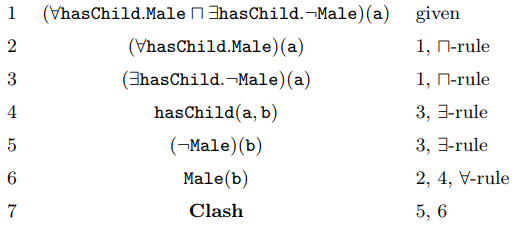
\includegraphics[width=0.6\textwidth]{Capitulos/Logicas/tableau}
		\caption{Exemplo de aplicação das regras de \textit{Tableau}}
	\end{figure}

Note que nesse exemplo não há uso da \textit{$ \sqcup $-rule}. Quando ela é usada, são criados dois ramos. Para que a fórmula seja insatisfazível, os dois devem resultar em choque (\textit{Clash}).

Para verificar que sentenças no estilo $ \texttt{C} \sqsubseteq \texttt{D} $ são válidas, deve ser verificada a satisfazibilidade de $ \texttt{C} \sqcap \neg \texttt{D} $. Se essa última for insatisfatível, a primeira é válida.
	\chapter{Revisão de Crenças}
	\chapter{Ferramentas Computacionais}
\label{chap:ferramentas}

\lettrine{O}{} interesse no estudo de Desenvolvimento de Ontologias, Lógicas de Descrição e Revisão de Crenças, deve-se, em parte, às aplicações computacionais que tais áreas possuem. Neste capítulo, algumas delas serão abordadas.

\section{OWL}

O final da década de 1990 foi a época em que surgiu a ideia de Web Semântica. Esse conceito, já consolidado hoje, seria uma parte da \textit{World Wide Web} onde é possível o trabalho cooperativo entre as máquinas e os seres humanos. Ele ocorre a partir dos significados que são dados aos conteúdos disponíveis na rede, para que haja compreensão por ambos os tipos de agentes \citep{ferramentasHerman}.

A fim de que alguma Linguagem de Representação fosse criada, a \href{https://www.w3.org}{W3C} (sigla para Consórcio para a \textit{World Wide Web}) fundou o "\textit{Web Ontology Working Group}", no início dos anos 2000  \citep{ferramentasGrupo}. 

Os primeiros rascunhos foram publicados em julho de 2002, e em fevereiro de 2004, a OWL (\textit{Web Ontology Language}) tornou-se o padrão recomendado pela W3C para o processamento de ontologias \citep{ferramentasReco}.

Em outubro de 2007, um novo grupo foi concebido para adicionar alguns recursos à linguagem. Dois anos depois, a W3C fez o lançamento da OWL 2, que seria compatível com editores e raciocinadores semânticos \citep{ferramentasOWLGrupo2}. Ela foi recomendada oficialmente pela W3C em dezembro de 2012 \citep{ferramentasOWLReco2}.

Abaixo estão algumas características das duas versões da OWL.

\subsection{OWL Web Ontology Language}

A primeira versão possui três sublinguagens \citep{ferramentasOWL1}. Cada uma possui suas particularidades:

\begin{itemize}
	\item \textit{Lite}: Sublinguagem mais simples, feita para hierarquias de classificação com restringimentos simples. Suporta restrições de cardinalidade simples (apenas 0 ou 1).  Foi demonstrado que OWL-Lite é equivalente a $ \mathcal{SHIF^{(D)}} $ \citep{ferramentasGrau}.
	\item DL: É equivalente a $ \mathcal{SHOIN^{(D)}} $. Oferece expressividade máxima evitando alguns problemas de decidibilidade. Inclui todos os construtores da OWL. Possui mais complexidade formal do que a sublinguagem \textit{Lite}.
	\item \textit{Full}: Versão mais completa, oferecendo expressividade máxima e a liberdade sintática do RDF, só que sem garantias computacionais. Nessa sublinguagem, pode acontecer de uma Classe ser tratada como uma coleção de indivíduos ou como um indivíduo, o que acarreta problemas de decidibilidade. Não corresponde a nenhuma lógica de descrição.
\end{itemize}

\subsection{OWL 2 Web Ontology Language}

A segunda versão também possui sublinguagens \citep{ferramentasOWL2}. Elas são:

\begin{itemize}
	\item EL: Corresponde à lógica $ \mathcal{EL} $++. Funciona bem para ontologias com muitas classes e/ou propriedades. Permite a existência de algoritmos de inferência polinimiais.
	\item QL: Baseada na lógica de descrição DL-\textit{Lite}, foi feita para aplicações em que o volume de instâncias é muito grande e que a consulta de dados é a tarefa mais realizada. Tais consultas podem até ser implementadas usando sistemas de bancos de dados convencionais.
	\item RL: Criada para ontologias que precisam de raciocínio escalável, ou seja, que são possivelmente grandes em número de instâncias, mas que precisam de uma sublinguagem que mantenha um bom poder expressivo. É baseada em uma lógica de descrição chamada DLP.
	\item DL: Assim como no lançamento anterior, oferece bastante expressividade, sem esbarrar em problemas de execução por causa da indecibilidade. Ela pode ser mapeada para a LD $ \mathcal{SROIQ^{(D)}} $. 
	\item \textit{Full}: Análoga à da primeira versão. Muito expressiva, porém, indecidível.
\end{itemize}

\section{\textit{Protégé}}

\begin{figure}
	\centering
	
\includegraphics[width=0.5\textwidth]{Capitulos/Ferramentas/protege}
	\caption{O logotipo do \textit{Protégé}.}
	\label{img:Protege}
\end{figure}

O \href{https://protege.stanford.edu}{\textit{Protégé}} é um editor semântico, compatível com a OWL 2. Ele foi desenvolvido pelo Centro de Pesquisa para Informática Biomédica da Universidade de Stanford, em colaboração com alguns programadores da Universidade de Manchester \footnote{\url{https://protege.stanford.edu/about.php}}. Sua primeira versão foi lançada em 1999, e a atual é de 2017. Seu logotipo está exibido na Figura \ref{img:Protege}

Seguindo os princípios do \textit{Software} Livre, ele é um arcabouço gratuito e de código aberto, feito para a construção de sistemas inteligentes, com o uso ou não de uma interface gráfica.

Assim como o ambiente de desenvolvimento integrado Eclipse, o \textit{Protégé} é bastante flexível porque é possível desenvolver uma grande variedade de \textit{plug-ins} para serem acoplados a ele.

Para exemplificar alguns recursos do \textit{Protégé}, será usada, como exemplo, parte da ontologia criada neste estudo:

\begin{itemize}
	\item Os conceitos: 
	\begin{itemize}
		\item \texttt{Musica} $ \equiv $ \texttt{Cancao} $ \sqcup $ \texttt{HinoNacional};
		\item \texttt{Pop} $ \sqsubseteq $ \texttt{Cancao};
		\item \texttt{EDM} $ \sqsubseteq $ \texttt{Cancao};
		\item \texttt{Pessoa} $ \equiv $ \texttt{Cantor} $ \sqcup $ \texttt{Compositor}.
	\end{itemize}
	\item As propriedades:
	\begin{itemize}
		\item \textbf{\texttt{canta}}, com domínio \texttt{Cantor} e contradomínio \texttt{Musica};
		\item \textbf{\texttt{cantadaPor}}, inversa da propriedade acima.
	\end{itemize}
	\item As instâncias e asserções:
	\begin{itemize}
		\item \texttt{MarinaAndTheDiamonds}, instância da classe \texttt{Cantor};
		\item \texttt{Primadonna}, instância da classe \texttt{Pop};
		\item \texttt{MarinaAndTheDiamonds \textbf{canta} Primadonna};
		\item \texttt{Froot}, instância da classe \texttt{Pop};
		\item \texttt{MarinaAndTheDiamonds \textbf{canta} Froot};
		\item \texttt{Disconnect}, instância da classe \texttt{EDM};
		\item \texttt{MarinaAndTheDiamonds \textbf{canta} Disconnect}.	
	\end{itemize}
\end{itemize}

No \textit{Protégé}, a ontologia fica como na Figura \ref{img:Representacao}.

\begin{figure}[H]
	\centering
	\begin{subfigure}{.3\textwidth}
		\centering
		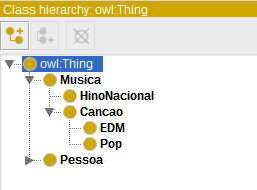
\includegraphics[width=0.95\linewidth]{Capitulos/Ferramentas/classes}
		\caption{A hierarquia das classes.}
	\end{subfigure}%
	\begin{subfigure}{.475\textwidth}
		\centering
		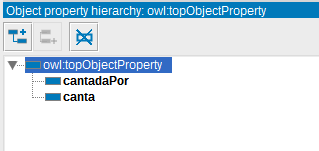
\includegraphics[width=0.95\linewidth]{Capitulos/Ferramentas/propriedades}
		\caption{As propriedades da ontologia.}
	\end{subfigure}
	\begin{subfigure}{.3\textwidth}
		\centering
		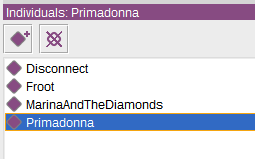
\includegraphics[width=0.95\linewidth]{Capitulos/Ferramentas/individuos}
		\caption{As instâncias definidas.}
	\end{subfigure}
	\caption{A representação da ontologia do \textit{Protégé}}
	\label{img:Representacao}
\end{figure}
 
\subsection{Raciocinadores}

Um aspecto interessante sobre esse arcabouço é o uso de \textit{plug-ins} de \textit{raciocínio}, como o HermiT \footnote{\url{http://www.hermit-reasoner.com/}}. A partir deles, é possível fazer inferências a partir dos axiomas lógicos que foram criados.

No fragmento da ontologia, temos que \texttt{MarinaAndTheDiamonds \textbf{canta} Primadonna}. É possível inferir que \texttt{Primadonna \textbf{cantadaPor} MarinaAndTheDiamonds}. O \textit{Protégé} consegue fazer isso com o auxílio do raciocinador, como exibido na Figura \ref{img:Raciocinador}.

\begin{figure}[H]
	\centering
	\begin{subfigure}{.5\textwidth}
		\centering
		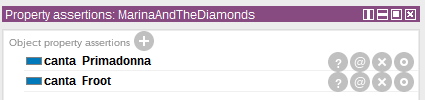
\includegraphics[width=0.9\linewidth]{Capitulos/Ferramentas/marinacanta}
		\caption{Músicas que \texttt{MarinaAndTheDiamonds} canta.}
	\end{subfigure}%
	\begin{subfigure}{.5\textwidth}
		\centering
		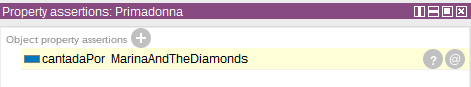
\includegraphics[width=0.95\linewidth]{Capitulos/Ferramentas/inferencia}
		\caption{Com o raciocinador, é mostrado quem canta Primadonna. O destaque indica inferência.}
	\end{subfigure}
	\caption{A asserção feita na construção da ontologia e a inferência feita.}
	\label{img:Raciocinador}
\end{figure}

\subsection{Buscas}

A partir de uma ontologia e de uma base de dados, é possível fazer buscas neste arcabouço, utilizando, entre várias linguagens de busca, o SPARQL.

SPARQL é um acrônimo recursivo para SPARQL \textit{Protocol and RDF Query Language}  \citep{ferramentasSPARQL}. Ele tem uma sintaxe que lembra a do SQL, e com seu uso, é possível tratar a ontologia como uma base de dados.  

Vale notar que as buscas funcionam apenas com a terminologia e as asserções gravadas no arquivo da ontologia. Para que as buscas funcionem sobre as inferências, é necessário exportá-las para um novo arquivo.

No exemplo utilizado, temos que \texttt{MarinaAndTheDiamonds} canta música de dois ritmos diferentes. Para descobrir quais são as músicas \texttt{Pop} que ela canta, podemos rodar uma consulta, como na mostrada na Figura \ref{img:Consulta}.

\begin{figure}[H]
	\centering
	\begin{subfigure}{.7\textwidth}
		\centering
		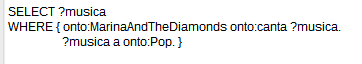
\includegraphics[width=0.95\linewidth]{Capitulos/Ferramentas/query}
		\caption{Fragmento da consulta para a pergunta. Note que o prefixo \texttt{onto} refere-se a definições dessa ontologia.}
	\end{subfigure}
	\begin{subfigure}{.7\textwidth}
		\centering
		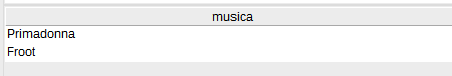
\includegraphics[width=0.95\linewidth]{Capitulos/Ferramentas/resultado}
		\caption{A consulta gera uma tabela com as músicas do ritmo \texttt{Pop} que \texttt{MarinaAndTheDiamonds} canta.}
	\end{subfigure}
	\caption{A consulta feita e seu resultado.}
	\label{img:Consulta}
\end{figure}
	\chapter{Implementação do \textit{Plug-In}}
	\chapter{Análise de desempenhos}
	\chapter*{Agradecimentos}
	
	\bibliographystyle{siam}
	\bibliography{monografia.bib}
	 
\end{document}